\documentclass{article}

% if you need to pass options to natbib, use, e.g.:
% \PassOptionsToPackage{numbers, compress}{natbib}
% before loading nips_2016
%
% to avoid loading the natbib package, add option nonatbib:
%\usepackage[nonatbib]{nips_2016}

%\usepackage{nips_2016}

% to compile a camera-ready version, add the [final] option, e.g.:
\usepackage[final]{nips_2016}

\usepackage[utf8]{inputenc} % allow utf-8 input
\usepackage[T1]{fontenc}    % use 8-bit T1 fonts
\usepackage{hyperref}       % hyperlinks
\usepackage{url}            % simple URL typesetting
\usepackage{booktabs}       % professional-quality tables
\usepackage{amsfonts}       % blackboard math symbols
\usepackage{nicefrac}       % compact symbols for 1/2, etc.
\usepackage{microtype}      % microtypography
\usepackage{amsmath}
\usepackage{mathtools}
\usepackage[usenames, dvipsnames]{color}
\usepackage{longtable}
\usepackage{caption}
\usepackage{subcaption}

\title{Recommending Subreddits to Reddit Users}

% The \author macro works with any number of authors. There are two
% commands used to separate the names and addresses of multiple
% authors: \And and \AND.
%
% Using \And between authors leaves it to LaTeX to determine where to
% break the lines. Using \AND forces a line break at that point. So,
% if LaTeX puts 3 of 4 authors names on the first line, and the last
% on the second line, try using \AND instead of \And before the third
% author name.

\author{
  %% examples of more authors
  %% \And
  %% Coauthor \\
  %% Affiliation \\
  %% Address \\
  %% \texttt{email} \\
  %% \AND
  %% Coauthor \\
  %% Affiliation \\
  %% Address \\
  %% \texttt{email} \\
  %% \And
  %% Coauthor \\
  %% Affiliation \\
  %% Address \\
  %% \texttt{email} \\
  %% \And
  %% Coauthor \\
  %% Affiliation \\
  %% Address \\
  %% \texttt{email} \\
}

\begin{document}
% \nipsfinalcopy is no longer used

\maketitle

\begin{abstract}
\textcolor{red}{[UPDATE OR DELETE]} In this paper we discuss the challenges of designing a recommenders system for Reddit.  We implement both collaborative filtering and content based approaches, [evaluating the effects of various normalization techniques and similarity metrics].  
\end{abstract}

\section{Introduction}
\label{sec:intro}
Reddit is a prominent social media platform which uses a bulletin board style website for users to share content with other users. In order to help users organize into communities of interest, Reddit hosts over 850,000 subreddits, with hundreds more being created each day.  A recommender system which finds related subreddits would help new users quickly explore similar subreddits and may help existing users find unexpected subreddits related to their interests. Alternatively, marketers may be interested in finding all subreddits related to their niche area to subscribe to or make posts in to promote their product. A robust recommender system may even help uncover communities participating in illegal activity which would otherwise seek to remain hidden, assisting authorities who are seeking to shut down subreddits that perpetuate hate speech or enable crime (such as child pornography, theft of digital media, or trafficking of illicit substances).

Recommender systems are broadly grouped into two strategies.  Content based systems focus on measuring similarity in the features of the item itself.  In contrast, collaborative filtering uses user feedback, either explicit (e.g. star ratings on Netflix) or implicit (e.g. a user’s viewing history), to find similarities between like-minded users.  The use of collaborative filtering methods based on implicit user feedback has grown in popularity with the increased passive tracking of user behavioral data, but can present challenges such as sparse and/or noisy data, ambiguous data interpretation (no negative ratings, mapping of behavior to preference may be unclear), and the "cold start" problem (unable to evaluate new users or items).  

\section{Data}
\label{sec:data}

\subsection{Data Collection}
\label{sec:feature-mapping}
In this paper, we focus on memory-based, collaborative filtering methods using implicit user feedback, although we attempt a limited implementation of content based, text similarity recommendations for a smaller subset of subreddits.  We use Reddit post and comment data from August 2016 made publicly available on Google BigQuery (7,591,689 posts and 69,654,819 comments by 3,698,088 unique users on 100,279 subreddits).\footnote{https://bigquery.cloud.google.com/table/fh-bigquery:reddit\_comments.2016\_08, https://bigquery.cloud.google.com/table/fh-bigquery:reddit\_posts.2016\_08} From this data set, we derived the following features:

\paragraph{Number of Posts} There are two ways in which users can contribute content to Reddit, either by making a top-level post or by commenting on a post.  The number of top-level posts a user makes to a subreddit can be a proxy for the degree to which that user is interested in that subreddit.  

\paragraph{Number of Comments} Similarly, number of comments can be used as an implicit indicator of user interest.  Comments are much more common than posts (by almost 10 to 1) and some users who never originate posts are nonetheless active commenters, so comments may provide more complete information on user preferences/behavior. 

\paragraph{Length of Comments} A raw count of posts or comments does not give any sense of the post/comment quality .  Length of comments could be one way to gain additional insight into the “value” of a comment, with the assumption that longer comments may indicate a higher degree of interest.  However, shorter comments do not necessarily indicate a lesser degree of interest, as brevity on Reddit is common and some subreddit cultures tend toward a short comment style.  Since post titles have a character limit of 300, the length of post titles would not be an indicator of interest.  

\paragraph{Post Scores} All posts and comments have a score (or number of points) based on the number of upvotes or downvotes it receives.  Reddit uses this score to determine which posts rise to the top of a subreddit home page or the top of the comments listed underneath each post.  The total number of points a user has received from all his or her posts on a particular subreddit can be a proxy for the “quality” or value of his or her contribution to that subreddit (in the opinion of other members of that subreddit community).  We infer that a user makes higher quality contributions to subreddits which he or she is more interested in.

\paragraph{Shared Users} We infer than subreddits which share a greater number of users (based on posting and commenting history) are more related, and for each subreddit pair we calculate the percent of users who posted or commented on both subreddits in August.  We use these results to conduct item-based collaborative, expecting that items will be easier to characterize than users (there are likely more similarities between two basketball subreddits than two basketball fans).  Since items are typically less dynamic and fewer in number than users, item-based collaborative filtering can also help to address scalability issues.

\paragraph{Text Similarity} In this content based approach, we consider the titles of posts in each subreddit and use term frequency-inverse document frequency (TF-IDF) to estimate similarity (see Section 2.3); similar methods could be applied to subreddit comments. Using the content of subreddits to generate recommendations would help to address the “cold start” problem, allowing users who do not have a post or comment history to find similar subreddits.  Although a new subreddit would not be evaluated until it has built up a post/comment history, this limitation is not necessarily negative, as it is not meaningful to recommend a subreddit which lacks any content.

\subsection{Data Preprocessing}\label{sec:data-prepros}
The Reddit data set is both large and inherently noisy, challenges common to many recommender systems which rely on implicit feedback.  In order to reduce data set to a more manageable size, we first removed known bots\footnote{Bots were identified by manually checking all those users with >3000 comments in one month and also by scraping /r/botWatcher for the names of all bots mentioned in the 500 most recent posts.  There are inevitably bots that remain unidentified in our data set, however we identified 955 bots (190 active) which accounted for 9.2\% of total posts and comments in August 2016.} and default subreddits\footnote{There are 49 default subreddits which all users are automatically subscribed to when they sign-up for a new account.  These subreddits are also linked at the top of every Reddit page and accounted for 17.6\% of all posts and comments in August 2016.}.  
%\textcolor{red}{[PLACEHOLDER - We further reduced the data set by only selecting those remaining users who posted to at least 10 subreddits or more.  Unless otherwise noted, this data set was used in all the following evaluations.]} 

After reducing the data set, the next critical step was to normalize the data in order to account for differences in user behavior.  For example, in the August 2016 Reddit data set, users made anywhere from 1 to over 10,000 comments in one month.  In order to compare across users and subreddits, we experimented with a number of different normalization, weighting, and segmentation techniques.

\paragraph{Gaussian Normalization} In order to account for differences in a user's average behavior (some users may contribute a large number of comments whereas others may only make a few comments) and variance within user behavior (some users may post about the same amount on all subreddits whereas others may disproportionately post to a few subredits), we apply a Gaussian normalization, subtracting each feature by the user's mean for that feature and dividing by the standard deviation: \begin{align*}
\hat{F}_{b}(a) = \frac{F_{b}(a) - \bar{F}_b}{\sqrt{\sum_{a}{(F_{b}(a) - \bar{F}_b)^2}}}
\end{align*}

where $\hat{F}_{b}(a)$ is the feedback for subreddit $a$ by user $b$ and $\bar{F}_b$ is the average feedback for user $b$.

\paragraph{Log Normalization} We also experiment with log normalization ($\hat{F}_{b}(a) = 1 + log(F_{b}(a))$) with the intuition that as a user's activity on a subreddit increases, the additional information gained by that increased activity diminishes.  For example, if user B makes 60\% of his posts to subreddit A, he is likely more interested in subreddit A than user C, who makes 30\% of his posts there, but not twice as interested.

%\paragraph{\textcolor{red}{Other stuff?} }
\paragraph{“TF-IDF-like” Weighting} In order to account for the fact that user activity on an extremely popular subreddit is not as informative as activity on a more niche subreddit in characterizing a user’s preferences, we experimented with weighting our features with an “IDF-like” term which is given by $log(\frac{N}{n_s})$ where $N$ is the number of users who posted or commented to any subreddit and $n_s$ is the number of users who posted or commented to the subreddit s.  TF-IDF is discussed in greater detail in the next section, but this term should have the effect of reducing the significance of a user's posts/comments on subreddits which have a large number of other users posting on it. 

\paragraph{Segmentation} Finally, we segmented our data set by the number of subreddits which each user posted or commented to (for example users who post to 2-4 subreddits, 4-15 subreddits, etc).  Users who are active on only a few subreddits may lead to abnormally high ratings and skew the similarity measures (a user who posts the same amount to two subreddits would give each subreddit his maximum rating).  By segmenting our data, we were able to select the best recommender for each category of user. 
%\textcolor{red}{please check this paragraph - I kind of made it up}

\subsection{Text processing}

Preprocessing text and generating text-based numeric features required additional considerations.  In order to show proof of concept, we created a smaller data set from the post titles of the 5,000 most posted to subreddits that had less than 100,000 posts in August 2016 and were not default subreddits.\footnote{This data set resulted in subreddits with between 163 and 73,577 posts in August 2016.  We were interested in active subreddits, but did not want to be overwhelmed by subreddits with an unusually high number of posts.  We selected post titles because each post title is limited in length and therefore easier to compare across subreddits and more computationally manageable.}   We then used a combination of regular expressions and packages from the Natural Language Toolkit (NLTK)\footnote{http://www.nltk.org/} to create a “bag of words” for each subreddit by removing all non-alphanumeric characters and capitalization, filtering for stop words, tokenizing those words that were greater than two characters, and applying a Porter stemmer. 

We use the TfidfVectorizer package from sklearn\footnote{http://scikit-learn.org/stable/modules/generated/sklearn.feature\_extraction.text.TfidfVectorizer.html} to transform our bag of words to a matrix of TF-IDF features.   TF-IDF is a well-known information retrieval weighting scheme which represents how significant a term is to a document in relation to how common that term is in the document and how rare that word is in the larger corpus of documents.  In our case, a document is the collection of all cleaned and tokenized titles posted on a single subreddit in August 2016 and the corpus of documents is the entire set of titles for all subreddits.  

We apply log normalization to the term frequency ($tf_{t,d}$) to account for our belief that multiple occurrences of a term have less significance as the number of occurrences increases.  The log normalized term frequency (${\hat{tf}_{t,d}}$), inverse document frequency ($idf_{t,N}$), and TF-IDF ($tfidf_{t,d,N}$) value for term $t$ in document $d$ are given by \begin{align*}
  {\hat{tf}_{t,d}} = \begin{cases}
                  1 + log(tf_{t,d}), & \text{if $tf_{t,d}$} > 0\\
                  0, & \text{otherwise}
              \end{cases} ; \text{      }    
    idf_{t,N} = log(\frac{N}{df_t}) 
\end{align*}
\begin{align*}
tfidf_{t,d,N} = {\hat{tf}_{t,d}} \times idf_{t,N}
\end{align*}

where $N$ is the number of documents in the corpus and $df_t$ is the number of documents in which the term $t$ appears.

We further apply $L2$ (Euclidean) normalization to the TF-IDF values such that $\hat{v} = \frac{v}{{\lVert{v}\lVert}_2}$.  Using this matrix of TF-IDF features, we compute pairwise cosine similarity by applying a linear kernel to the already $L2$-normalized data.


\section{Recommender Architecture}\label{sec:rec-arch}

To build our recommenders, we use the Java package Mahout. The code
used to test the various algorithms in our package and to implement
our subreddit recommender can be found on our Github repo page\footnote{https://github.com/qqliu/subreddit-recommendations}. The specific 
architectures that are used are the Mahout collaborative filtering and item-based recommendation algorithms. 
We use the following set of collaborative filtering similarity algorithms: 
Pearson Correlation, Euclidean Distance, Log Likelihood, Tanimoto Coefficient, and Uncentered Cosine. 
Once these similarities are calculated, we further use a neighborhood algorithm to 
determine the nearest neighbors. This algorithm either finds the nearest
$n$ neighbors or a threshold similarity where if the similarity of a specific user is
greater than a score, then we include the items liked by these
users. We briefly explain
the pitfalls and advantages of each of these algorithms below. Furthermore, we evaluate the 
accuracy of these algorithms by performing a series of hold-out experiments both by using the 
evaluator code provided by the Mahout package and by implementing our own testing suite.

\subsection{Similarity Measures}

\paragraph{Pearson Correlation}

The Pearson Correlation similarity measure looks at how similar data variation curves are from each other. 
Specifically, given two items, we compute the following as the Pearson Correlation: \begin{align*}
r_{X, Y} = \frac{\sum_{x_i, y_i \in X, Y} (x_i - \overline{x})(y_i - \overline{y})}{\sqrt{\sum_{i = 1}^n (x_i - \overline{x})^2}\sqrt{\sum_{i=1}^n (y_i - \overline{y})^2}}
\end{align*}

where $x_i \in X$ and $y_i \in Y$ are data samples of $X$ and $Y$ respectively, $n$ is the total number of samples,
and $\overline{x}$ and $\overline{y}$ are the means of all samples in $X$ and $Y$. In terms of users and 
item preference ratings, $X$ is the set of item preferences of user $X$ and $Y$ is the set of item 
preferences of user $Y$. 

One advantage of this similarity measure is that the data is normalized to look at proportionality trends between 
pairs of user preference vectors (essentially looking at the trends and the tendency of the values to move 
together proportionally) rather than the actual values. For instance, points on two parallel lines have Pearson 
correlation $1$ \textcolor{red}{NOTE: Check this.}. Therefore, this similarity measure is robust against user preferences that have different means and variances among different users. For instance, for users who
posted to more than $25$ subreddits, the Pearson correlation similarity measure performed much
better than all other similarity measures\textcolor{red}{NOTE: Check this}.

The major disadvantage of this similarity measure is that users who only rated one item or rated all items the 
same rating will have covariance $0$ which prevents any Mahout collaborative filtering algorithm based 
on this measure from making a recommendation. Other similarity measures mentioned below will be better able
to handle such sparsity of data. We see this effect in our results for data that includes users who have
only made comments in $2 \leq n \leq 3$ subreddits (see Section~\ref{2-3-users}). 
Using Pearson correlation, the predicted values matched poorly
with the actual values. Furthermore, by removing the top ranked item, the data becomes too sparse for the recommendation algorithm to retrieve any meaningful recommendations (at least by the precision and recall measures).

\paragraph{Euclidean Distance}

This measure assumes items are dimensions and each user is a point in $\mathrm{R}^n$ where $n$ is the total
number of ratable items. Then, for any two users, we compute the Euclidean distance between the two users.
The similarity $r$ between two users, $X$ and $Y$, is calculated by the following equation: \begin{align*}
r_{X, Y} = \frac{\sqrt{n}}{1 + \sqrt{\sum_{x_i, y_i \in X, Y} (x_i - y_i)^2}}
\end{align*}

where the $\sqrt{n}$ is meant to help correct against users with more ratings automatically receiving lower scores. 
(In fact, more similar ratings should indicate \emph{greater} similarity between users.) Unlike the Pearson correlation,
the Euclidean distance metric does not have a problem with sparse data sets, although this similarity measure 
performs better when all points have approximately the same number of dimensions. (As we can see in Section
~\ref{sec:set-com-posts}. \textcolor{red}{Check this!})

\paragraph{Spearman Correlation}

This measure is the same implementation as the Pearson correlation similarity except all preferences are ranked and the 
rankings are used to compute the correlation value.

\paragraph{Log Likelihood}

This similarity measure computes the log likelihood of two ratings appearing together using the following equation: given two items, $i$ and $j$, we can compute the number of users that have ratings for $i$ and $j$, $k_{i,j}$, the number of users
who rated $i$ but not $j$, $k_{i,\overline{j}}$, the number of users who have rated $j$ but
not $i$, $k_{\overline{i}, j}$, and the number of users who have rated neither $i$ or $j$, 
$k_{\overline{i}, \overline{j}}$ (i.e. the values are in a coocurrence matrix, $K$). 
The log likelihood of $i$ and $j$ occurring together is
then:\begin{align*}
r_{i, j} = 2 \left(\sum_{l \in {i, \overline{i}}, m \in {j, \overline{j}}} k_{l, m} \right)(H(K) - H(K_i) - H(K_j))
\end{align*}

where $N = \sum_{l \in {i, \overline{i}}, m \in {j, \overline{j}}} k_{l, m}$, $H = \sum_{l \in {i, \overline{i}}, m \in {j, \overline{j}}}\left(k/N \log(k/N)\right)$, and $K_i$ is a vector of row sums of $K$ and $K_j$ is a vector of column sums. 

The main advantage of this measure is that it allows for similarity measures based on boolean preferences or user
interactions with items that do not have clear preferences. In fact, this similarity computes how \emph{unlikely} it is
for two probability distributions to be independent (i.e. how likely they are dependent), so higher values indicate 
greater dependence and greater similarity.

\paragraph{Tanimoto Coefficient}

\textcolor{red}{Clarify?} This measure computes the
fraction that preference user $X$ and user $Y$ share a relation with the same items:\begin{align*}
r_{X, Y} = \frac{\sum_i X_i \wedge Y_i}{\sum_i X_i \vee Y_i}
\end{align*}

This is a simpler similarity than the log likelihood measure and returns a value in $[0, 1]$. 

\paragraph{Uncentered Cosine}

If we imagine a user list of preferences for items is a vector in space, then the uncentered cosine similarity computes
the cosine of the angle between these vectors. If the data is normalized, then this similarity measure calculates the
same number as the Pearson correlation measure. Therefore, we only present a few results in Section~\ref{sec:results} related to this measure.

\subsection{User Neighborhood Algorithms}

\paragraph{Nearest N Neighbors} This returns the nearest $N$ users (i.e. users with the highest similarity to the current
user) and bases recommendations on the nearest $N$ users. In our evaluations, we vary the neighborhood size to 
determine the optimum neighborhood size. 

\paragraph{Threshold-based neighborhood} Picks all users who have similarity greater than threshold $k$. 

\section{Results}\label{sec:results}

We use three forms of evaluation to determine the effectiveness of each of the methods we test: two quantitative
methods and one qualitative method. The two quantitative methods we use are two types of holdout experiments.
In the first instance, we hold a random portion of the training data set as the testing set. Then, we compute the 
predicted preference values for each of the item-user pairs that was "held-out" and compute the error between
the predicted preference values and the expected preference values (i.e. the actual preference values). We
also compute the precision and recall of each evaluation based on how many of the returned values
were held-out. Let $p$ be the precision value and $r$ be the recall value:\begin{align*}
p = \frac{|\left\{ \text{relevant items} \right\} \cap \left\{\text{retrieved items}\right\}|}{|\left\{\text{retrieved items}\right\}|}
\end{align*}
\begin{align*}
r = \frac{|\left\{ \text{relevant items} \right\} \cap \left\{\text{retrieved items}\right\}|}{|\left\{\text{relevant items}\right\}|}
\end{align*} 

where $\left\{relevant items\right\}$ is the set items that were ``held-out'' by the hold-out experiment and $\left\{retrieved items\right\}$ is the set of items returned as recommendations to users by the algorithm.

For the qualitative test, we retrieved $60$ sets of $7$ recommendations for $60$ users and $40$ sets of randomly
generated recommenders for $40$ ``users'' and evaluated the similarity between items in the set qualitatively by 5 
people. More details about the method is provided in Section~\ref{sec:qualitative-evaluations}. 

\subsection{Preference Values and Feature Mappings}

Here, we explain our test results for the various feature mappings we used in Section~\ref{sec:feature-mapping}. 
For each type of feature mapping, we test all algorithms mentioned in Section~\ref{sec:rec-arch} by varying user
similarity measures and nearest neighbor parameters and threshold values. For these evaluations, 
we perform both types of quantitative evaluations. For determining the error between predicted preferences and 
the actual preferences based on the feature mappings, we use the root-mean-square error calculation and the average
absolute value difference. Furthermore, we normalize the differences between feature values by dividing by the average
amount each user rating differs from the mean of each user preference vector so that we can compare
how different each predicted value is from a difference of one level of rating.\textcolor{red}{I do not understand this last sentence}) The characteristics of each dataset is
shown in Table~\ref{dataset-chars}.

\begin{table}
    \begin{tabular}{ |p{2.5cm}|p{2cm}|p{3cm}|p{3cm}|p{2.5cm}|}
    \hline
    File Type& Mean of User Means & Standard Deviation of User Means & Feature Value $-$ User Mean & RMS of Feature Val $-$ User Mean\\ \hline\hline
    Num Comments (7632154)& 0.587 & 0.260 & 0.209 & 0.279 \\ \hline
    Num Posts (1603887)& 0.713 & 0.189 & 0.137 & 0.213 \\ \hline
    Num Posts TF-IDF (1497880) & 0.771 & 0.161 &  0.176 & 0.220 \\ \hline
    Num Comments TF-IDF (4715952) & 0.713 & 0.189 & 0.216 & 0.262 \\ \hline
    Avg Comment Length (7632044) & 0.594 & 0.187 & 0.229 & 0.283 \\ \hline
    Posts Score (1434089) & 0.638 & 0.238 & 0.275 & 0.336 \\
    \hline
    \end{tabular}
    \caption{Details about each file. We compute the mean and standard deviation of the mean of each user vector,
     the mean difference between each user feature value and the mean of that user's feature values, and the root mean
     square of the different between each user feature value and the mean of the user's feature values. 
     Each file is normalized by dividing by the maximum feature value for each user.}\label{dataset-chars}
\end{table}

We compare our results to a randomly generated file with $2,000,000$ lines. For the random file, we choose random 
choose user and item pairs such that the expected number of ratings per user is $10$. We created a set of $20,000$ items
where the items for each user is chosen uniformly at random from the set of total items. Furthermore, we compute a 
rounded two-decimal rating from a Gaussian distribution with mean $0.7$ and standard deviation $0.17$. Using this
file of random user ratings and item pairs, none of the models are able to train, meaning that all the files
we provide have some form of correlation/are able to train a model whereas the random file cannot.

The results we obtain can be found in the following table:

\subsection{Feature Mapping and Recommendation Quantitative Results}\label{sec:feature-mapping}

We considered the $6$ different feature mappings considered in Section~\ref{sec:feature-mapping}. For each of these
feature mapping procedures, we test the $5$ similarity measures, Pearson, Euclidean Distance, Log Likelihood, 
Spearman Correlation, and Tanimoto Coefficient to determine the root-mean-square error between the predicted 
preference of each user for a given subreddit that was held-out by the hold-out test. The lower the score, the 
greater the chance that preferences calculated by using the similarity measure matches preferences expressed 
by the user by \emph{using a specific feature map}. We use the precision and recall to determine how correlated 
user preferences are from this particular feature mapping. Note that since we use $0.9$ of the data for training
and $0.01$ of the data for testing RMS error and $0.0001$ of the users for testing precision and recall, there
could be variations in the number of users that are tested depending on how much data there is. However,
we believe that this should not greatly affect our results. The number of users used for testing can be found in
Table~\ref{results-basic}.

We found through our tests that the feature map that resulted in the greatest precision and recall was the 
number of posts made to a particular subreddit. As can be seen in Fig.~\ref{fig:feature-map}, for instance,
for $50$ neighbors and using Pearson correlation, the precision is $0.5$ and the recall is $0.1$ which 
outperforms all other feature maps when using a neighborhood of $50$ and any of the other
similarity algorithms. For both the NC-TFIDF and NP-TFIDF feature, maps, we see  a performance
that is worse than the original NC and NP datasets in terms of recall. We use the RMS error to 
determine the best similarity measure for each dataset and the precision and recall to compare 
performance across datasets.

We believe that the number of posts performs the best out of all datasets because posting in a subreddit
shows greater preference for the subreddit than commenting on a subreddit. Furthermore, users
make fewer posts to fewer subreddits resulting in less noise than a dataset that has users
make the same ratings for a lot of different items. 

\begin{figure}[h]
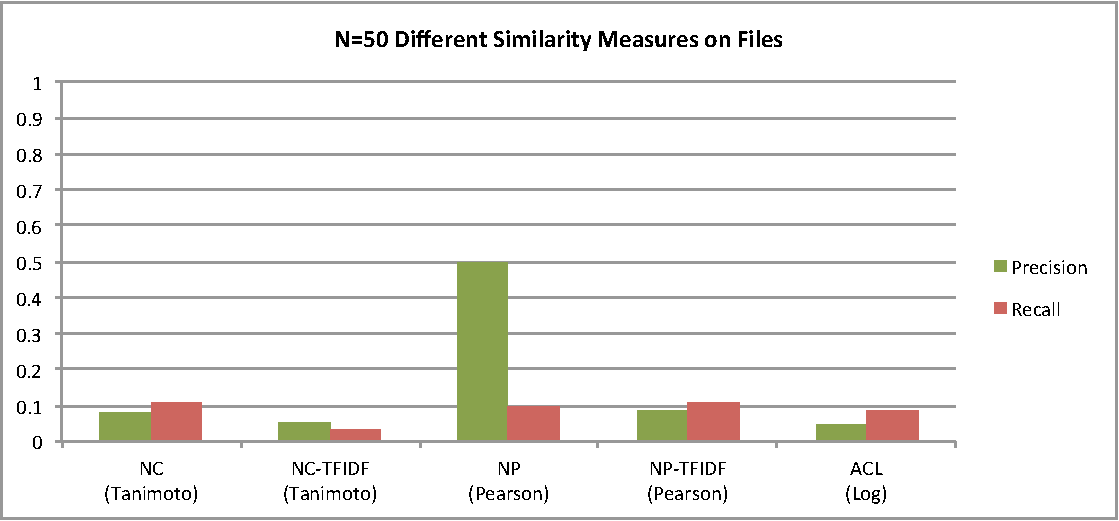
\includegraphics[width=\textwidth]{img/sim-on-files.pdf}
\caption{Precision and recall due to different similarity measures that resulted in smallest
root-mean-squared error.}\label{fig:feature-map}
\end{figure} 

\begin{figure}[h]
\centering
\begin{subfigure}{.4\textwidth}
  \centering
  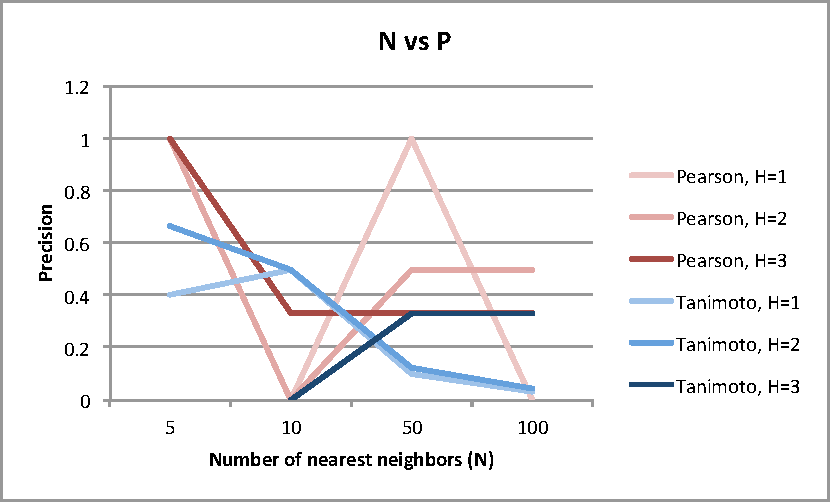
\includegraphics[width=\linewidth]{img/nvp.pdf}
  \label{fig:nvp}
\end{subfigure}%
\begin{subfigure}{.4\textwidth}
  \centering
  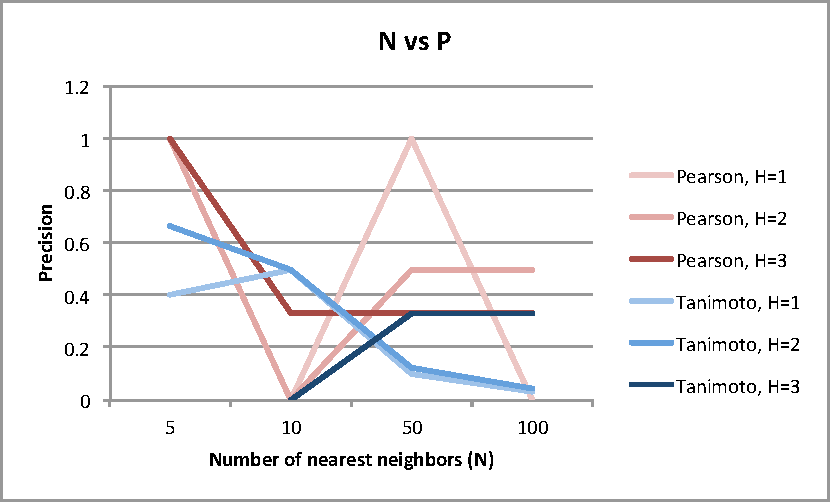
\includegraphics[width=\linewidth]{img/nvp.pdf}
  \label{fig:tvp}
\end{subfigure}
\begin{subfigure}{.4\textwidth}
  \centering
  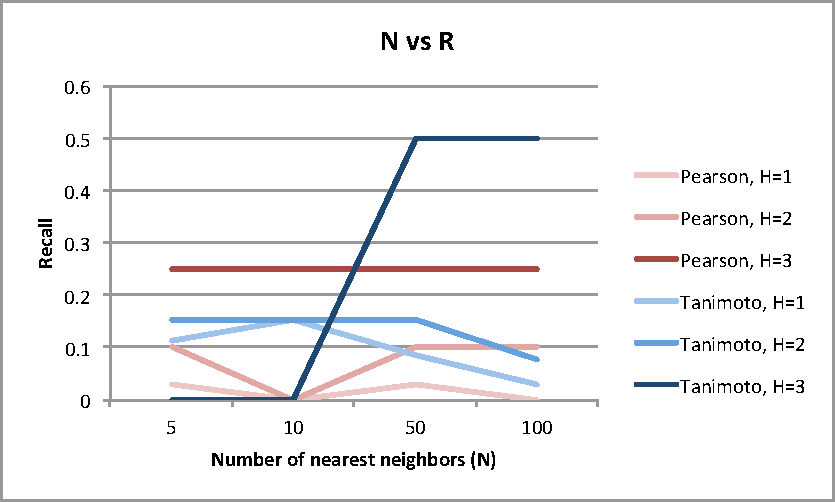
\includegraphics[width=\linewidth]{img/nvr.pdf}
  \label{fig:nvr}
\end{subfigure}%
\begin{subfigure}{.4\textwidth}
  \centering
  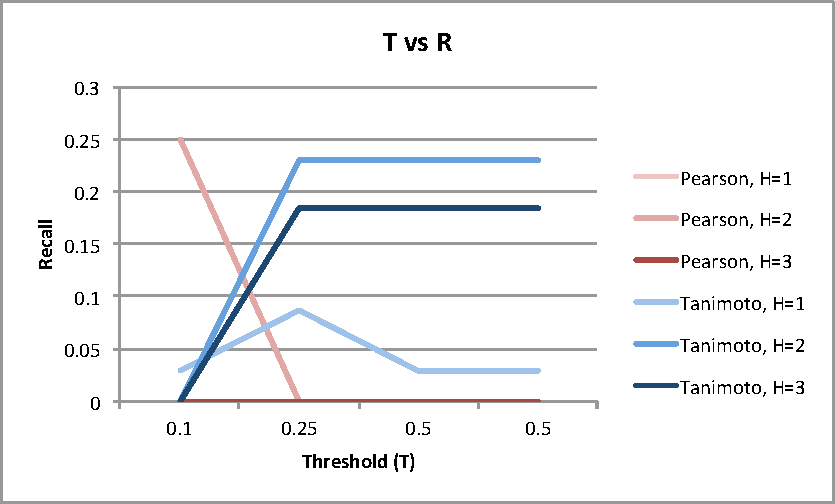
\includegraphics[width=\linewidth]{img/tvr.pdf}
  \label{fig:tvr}
\end{subfigure}
\caption{Precision and recall due to different similarity measures: Pearson correlation and
Tanimoto coefficient.}\label{fig:learning-rate-hidden-layers}
\end{figure}

\subsection{Different Normalization Results}\label{sec:different-normalization}

We use the normalization methods mentioned in Section~\ref{sec:data-prepros}. We see that both NC-TFIDF and NP-TFIDF perform worse than NC and NP in terms of precision and recall. We can see these 
results in Fig.~\ref{tfid-f-p} where we see the precision and recall of NP-TFIDF and NP given user neighborhoods
$N =10, 50$ and $T = 0.1, 0.5$ and varying $H$. However, we see that both the logarithm normalization 
perform better than the original dataset as can be seen In Fig.~\ref{varying-log-gaussian}, while (as expected), 
the Gaussian normalization performs as well (approximately the same) as the original. 
 
\subsection{Segmentation of Comments and Posts}\label{sec:set-com-posts}

We find that segmenting the comments and posts into smaller groups and then, using a different similarity measure
and collaborative filtering algorithm for each segment performed better by both our quantitative and qualitative
measure than by feeding a large data set \emph{that is not segmented} into a recommender. For this procedure, 
we test against the NC dataset since it contains the most number of ratings and the greatest variance
in terms of the number of subreddits that users contributed to. We segment the ratings into the following segments: 
ratings from users who contribute to [2, 3] subreddits, [4, 6] subreddits, [6, 15] subreddits, [15, 25], subreddits, [25, 50] 
subreddits, and, finally, [50-1000] subreddits. We see that as we believed, segmenting the dataset
resulted in greater precision and recall than the original NC dataset. Furthermore, different similarity 
measures and recommender algorithm parameters performed better in each segment. 

\subsubsection{Users who commented or posted to $2$ or $3$ subreddits}\label{2-3-users}

Here, we see that the Tanimoto coefficient performs better than the Pearson coefficient (also 
better than any other similarity measures). 

\subsubsection{Users who commented or posted to more than $25$ subreddits}\label{more-than-25}

\subsection{Qualitative Evaluations}\label{sec:qualitative-evaluations}

\begin{longtable}{ |p{1.7cm}|p{1.9cm}|p{1.5cm}|p{1.5cm}|p{0.75cm}|p{0.75cm}|p{0.75cm}|p{0.75cm}|p{1.5cm}|p{1.5cm}|}
    \hline
    File & Sim Measure & \# Training & \# Testing & $N$ & $T$ & $H$ & RMS Err & Precision & Recall \\ \hline\hline
    NC & Pearson & 4244356 & 47159 & 50 & N/A & N/A & 0.398 & N/A & N/A  \\ \hline
    NC  & Euc Dist & 4244356 & 47159 & 50 & N/A & N/A & 0.403 & N/A & N/A   \\ \hline
    NC  & Log & 4244356 & 47159  & N/A &  50 & N/A& 0.399 & N/A & N/A  \\ \hline
    NC  & Spearman & 4244356 & 47159  & 50 & N/A & 0.404 & N/A & N/A & N/A \\ \hline
    NC  & Tanimoto & 4244356 & 47159 & 50 & N/A& N/A & 0.391 & N/A & N/A \\ \hline
    NC  & Log & 4244356 & 47159 & 50 & N/A& N/A & 0.301 (Avg) & N/A & N/A \\ \hline
    NC  & Tanimoto & 4244356 & 4719 & 50 & N/A & N/A & 0.316 (Avg) & N/A & N/A \\ \hline
    
    NC  & Pearson & 4244356 & 471 & 50 & N/A  & 2 & N/A & 0.029 & 0.0357  \\ \hline
    NC  & Euc Dist & 4244356 & 471 & 50 & N/A  & 2 & N/A & 0.016 & 0.032   \\ \hline
    NC  & Log & 4244356 & 471& 50 & N/A & 2 & N/A & 0.063 & 0.041  \\ \hline
    NC  & Spearman & 4244356 & 471 & 50 & N/A  & 2 & N/A &0.046 & 0.070 \\ \hline
    NC  & Tanimoto & 4244356 & 471 & 50 & N/A  & 2 & N/A & 0.078 & 0.106 \\ \hline
    
    NC-TFIDF & Pearson & 4244356 & 47159 & 10 & N/A & N/A & 0.394 & N/A & N/A  \\ \hline
    NC-TFIDF  & Euc Dist & 4244356 & 47159 & 10 & N/A & N/A & 0.342 & N/A & N/A   \\ \hline
    NC-TFIDF  & Log & 4244356 & 47159  & N/A &  10 & N/A& 0.353 & N/A & N/A  \\ \hline
    NC-TFIDF  & Spearman & 4244356 & 47159  & 10 & N/A & 0.489 & N/A & N/A & N/A \\ \hline
    NC-TFIDF  & Tanimoto & 4244356 & 47159 & 10 & N/A& N/A & 0.350 & N/A & N/A \\ \hline
    NC-TFIDF  & Log & 4244356 & 47159 & 10 & N/A& N/A & 0.279 (Avg) & N/A & N/A \\ \hline
    NC-TFIDF  & Tanimoto & 4244356 & 4719 & 10 & N/A & N/A & 0.289 (Avg) & N/A & N/A \\ \hline
    
    NC-TFIDF  & Pearson & 4244356 & 471 & 10 & N/A  & 2 & N/A & 0.0 & 0.0  \\ \hline
    NC-TFIDF  & Euc Dist & 4244356 & 471 & 10 & N/A  & 2 & N/A & 0.230 & 0.291   \\ \hline
    NC-TFIDF  & Log & 4244356 & 471& 10 & N/A & 2 & N/A & 0.063 & 0.041  \\ \hline
    NC-TFIDF  & Spearman & 4244356 & 471 & 10 & N/A  & 2 & N/A &0.037 & 0.065 \\ \hline
    NC-TFIDF  & Tanimoto & 4244356 & 471 & 10 & N/A  & 2 & N/A & 0.0 & 0.0 \\ \hline
    
    NC-TFIDF & Pearson & 4244356 & 47159 & 50 & N/A & N/A & 521 & N/A & N/A  \\ \hline
    NC-TFIDF  & Euc Dist & 4244356 & 47159 & 50 & N/A & N/A & 0.343 & N/A & N/A   \\ \hline
    NC-TFIDF  & Log & 4244356 & 47159 &  50 & N/A & N/A & 0.356 & N/A & N/A  \\ \hline
    NC-TFIDF  & Spearman & 4244356 & 47159 & 50 & N/A & N/A & 399 & N/A & N/A \\ \hline
    NC-TFIDF  & Tanimoto & 4244356 & 47159 & 50 & N/A& N/A & 0.362 & N/A & N/A \\ \hline
    NC-TFIDF  & Log & 4244356 & 47159 & 50 & N/A& N/A & 0.300 (Avg) & N/A & N/A \\ \hline
    NC-TFIDF  & Tanimoto & 4244356 & 47159 & 50 & N/A & N/A & 0.315 (Avg) & N/A & N/A \\ \hline
    
    NC-TFIDF  & Pearson & 4244356 & 471 & 50 & N/A  & 2 & N/A & 0.017 & 0.031  \\ \hline
    NC-TFIDF  & Euc Dist & 4244356 & 471 & 50 & N/A  & 2 & N/A &0.012 & 0.012   \\ \hline
    NC-TFIDF  & Log & 4244356 & 471 & 50 & N/A & 2 & N/A & 0.015 & 0.014  \\ \hline
    NC-TFIDF  & Spearman & 4244356 & 471& 50 & N/A  & 2 & N/A &0.0 & 0.0 \\ \hline
    NC-TFIDF  & Tanimoto & 4244356 & 471 & 50 & N/A  & 2 & N/A & 0.048 & 0.031 \\ \hline
   
    NC-TFIDF & Pearson & 4244356 & 47159 & N/A & 0.1 & N/A & 0.278 & N/A & N/A  \\ \hline
    NC-TFIDF  & Euc Dist & 4244356 & 47159 & N/A & 0.1 & N/A & 0.336 & N/A & N/A   \\ \hline
    NC-TFIDF  & Log & 4244356 & 47159 & N/A &  N/A & 0.1 & 0.341 & N/A & N/A  \\ \hline
    NC-TFIDF  & Spearman & 4244356 & 47159 & N/A & 0.1 & N/A & 0.268 & N/A & N/A \\ \hline
    NC-TFIDF  & Tanimoto & 4244356 & 47159 & N/A & 0.1 & N/A & 0.344 & N/A & N/A \\ \hline
    NC-TFIDF  & Log & 4244356 & 47159 & N/A & 0.1 & N/A & 0.272 (Avg) & N/A & N/A \\ \hline
    NC-TFIDF  & Tanimoto & 4244356 & 47159 & N/A & 0.1 & N/A & 0.294 (Avg) & N/A & N/A \\ \hline
    
    NC-TFIDF  & Pearson & 4244356 & 471 & N/A & 0.1 & 2 & N/A & 0.0 & 0.0  \\ \hline
    NC-TFIDF  & Euc Dist & 4244356 & 471 & N/A & 0.1 & 2 & N/A &0.0 & 0.0   \\ \hline
    NC-TFIDF  & Log & 4244356 & 471 & N/A & 0.1 & 2 & N/A & 0.0 & 0.0  \\ \hline
    NC-TFIDF  & Spearman & 4244356 & 471 & N/A & 0.1 & 2 & N/A &0.023 & 0.043 \\ \hline
    NC-TFIDF  & Tanimoto & 4244356 & 471 & N/A & 0.1 & 2 & N/A & 0.0 & 0.0 \\ \hline
    
    NC-TFIDF & Pearson & 4244356 & 47159 & N/A & 0.5 & N/A & 0.272 & N/A & N/A  \\ \hline
    NC-TFIDF  & Euc Dist & 4244356 & 47159 & N/A & 0.5 & N/A & 0.323 & N/A & N/A   \\ \hline
    NC-TFIDF  & Log & 4244356 & 47159 & N/A &  N/A & 0.5 & 0.333 & N/A & N/A  \\ \hline
    NC-TFIDF  & Spearman & 4244356 & 47159 & N/A & 0.5 & N/A & 0.317 & N/A & N/A \\ \hline
    NC-TFIDF  & Tanimoto & 4244356 & 47159 & N/A & 0.5 & N/A & 0.327 & N/A & N/A \\ \hline
    NC-TFIDF  & Log & 4244356 & 47159 & N/A & 0.5 & N/A & 0.282 (Avg) & N/A & N/A \\ \hline
    NC-TFIDF  & Tanimoto & 4244356 & 47159 & N/A & 0.5 & N/A & 0.266 (Avg) & N/A & N/A \\ \hline
    
    NC-TFIDF  & Pearson & 4244356 & 471 & N/A & 0.5 & 2 & N/A & 0.0 & 0.0  \\ \hline
    NC-TFIDF  & Euc Dist & 4244356 & 471 & N/A & 0.5 & 2 & N/A &0.0 & 0.0   \\ \hline
    NC-TFIDF  & Log & 4244356 & 471 & N/A & 0.5 & 2 & N/A & 0.0 & 0.0  \\ \hline
    NC-TFIDF  & Spearman & 4244356 & 471 & N/A & 0.5 & 2 & N/A &0.023 & 0.043 \\ \hline
    NC-TFIDF  & Tanimoto & 4244356 & 471 & N/A & 0.5 & 2 & N/A & 0.0 & 0.0 \\ \hline
    
    NP & Pearson & 6868938 & 76321 & 5 &  N/A & N/A & 0.999 & N/A & N/A  \\ \hline
    NP & Euc Dist & 6868938 & 76321 & 5 & N/A & N/A & 0.418 & N/A & N/A   \\ \hline
    NP & Log & 6868938 & 76321 & 5 &  N/A & N/A & 0.405 & N/A & N/A  \\ \hline
    NP & Spearman & 6868938 & 76321 & 5 & N/A & N/A & 0.167 & N/A & N/A \\ \hline
    NP & Tanimoto & 6868938 & 76321 & 5 & N/A & N/A & 0.269 & N/A & N/A \\ \hline
    NP & Log & 6868938 & 76321 & 5 & N/A & N/A & 0.203 (Avg) & N/A & N/A \\ \hline
    NP & Tanimoto & 6868938 & 76321 & 5 & N/A & N/A & 0.254 (Avg) & N/A & N/A \\ \hline
    
    NP & Pearson & 6868938 & 763 & 5 &  N/A & 1 & N/A & 1.0 & 0.031  \\ \hline
    NP & Euc Dist & 6868938 & 763 & 5 & N/A & 1 & N/A &0.231 & 0.071   \\ \hline
    NP & Log & 6868938 & 763 & 5 &  N/A & 1 & N/A & 0.2 & 0.029  \\ \hline
    NP & Spearman & 6868938 & 763 & 5 & N/A & 1 & N/A &0.0 & 0.0 \\ \hline
    NP & Tanimoto & 6868938 & 763 & 5 & N/A & 1 & N/A & 0.4 & 0.114 \\ \hline
    
    NP & Pearson & 6868938 & 763 & 5 &  N/A & 2 & N/A & 1.0 & 0.1  \\ \hline
    NP & Euc Dist & 6868938 & 763 & 5 & N/A & 2  & N/A &0.3 & 0.167   \\ \hline
    NP & Log & 6868938 & 763 & 5 &  N/A & 2  & N/A & 0.333 & 0.0714  \\ \hline
    NP & Spearman & 6868938 & 763 & 5 & N/A & 2  & N/A &0.0 & 0.0 \\ \hline
    NP & Tanimoto & 6868938 & 763 & 5 & N/A & 2  & N/A & 0.667 & 0.153 \\ \hline
    
    NP & Pearson & 6868938 & 763 & 5 &  N/A & 3 & N/A & 1.0 & 0.25  \\ \hline
    NP & Euc Dist & 6868938 & 763 & 5 & N/A &  3 & N/A &0.0 & 0.0   \\ \hline
    NP & Log & 6868938 & 763 & 5 &  N/A &  3 & N/A & NaN & 0.0  \\ \hline
    NP & Spearman & 6868938 & 763 & 5 & N/A &  3 & N/A &0.0 & 0.0 \\ \hline
    NP & Tanimoto & 6868938 & 763 & 5 & N/A &  3 & N/A & NaN & 0.0 \\ \hline
    
    NP & Pearson & 6868938 & 76321 & 10 &  N/A & N/A & 0.999 & N/A & N/A  \\ \hline
    NP & Euc Dist & 6868938 & 76321 & 10 & N/A & N/A & 0.416 & N/A & N/A   \\ \hline
    NP & Log & 6868938 & 76321 & 10 &  N/A & N/A & 0.374 & N/A & N/A  \\ \hline
    NP & Spearman & 6868938 & 76321 & 10 & N/A & N/A & 0.118 & N/A & N/A \\ \hline
    NP & Tanimoto & 6868938 & 76321 & 10 & N/A & N/A & 0.295 & N/A & N/A \\ \hline
    NP & Log & 6868938 & 76321 & 10 & N/A & N/A & 0.199 (Avg) & N/A & N/A \\ \hline
    NP & Tanimoto & 6868938 & 76321 & 10 & N/A & N/A & 0.281 (Avg) & N/A & N/A \\ \hline
    
    NP & Pearson & 6868938 & 763 & 10 &  N/A & 1 & N/A & 0.0 & 0.0  \\ \hline
    NP & Euc Dist & 6868938 & 763 & 10 & N/A & 1 & N/A &0.097 & 0.071   \\ \hline
    NP & Log & 6868938 & 763 & 10 &  N/A & 1 & N/A & 0.214 & 0.088  \\ \hline
    NP & Spearman & 6868938 & 763 & 10 & N/A & 1 & N/A &0.0 & 0.0 \\ \hline
    NP & Tanimoto & 6868938 & 763 & 10 & N/A & 1 & N/A & 0.5 & 0.154 \\ \hline
    
    NP & Pearson & 6868938 & 763 & 10 &  N/A & 2 & N/A & 0.0 & 0.0  \\ \hline
    NP & Euc Dist & 6868938 & 763 & 10 & N/A &  2 & N/A &0.125 & 0.167   \\ \hline
    NP & Log & 6868938 & 763 & 10 &  N/A &  2 & N/A & 0.083 & 0.071 \\ \hline
    NP & Spearman & 6868938 & 763 & 10 & N/A &  2 & N/A & 0.0 & 0.0 \\ \hline
    NP & Tanimoto & 6868938 & 763 & 10 & N/A &  2 & N/A & 0.5 & 0.154 \\ \hline
    
    NP & Pearson & 6868938 & 763 & 10&  N/A & 3 & N/A & 0.333 & 0.25  \\ \hline
    NP & Euc Dist & 6868938 & 763 & 10 & N/A & 3  & N/A &0.333 & 0.111   \\ \hline
    NP & Log & 6868938 & 763 & 10 &  N/A & 3  & N/A & 0.0 & 0.0  \\ \hline
    NP & Spearman & 6868938 & 763 & 10 & N/A & 3  & N/A &0.0 & 0.0 \\ \hline
    NP & Tanimoto & 6868938 & 763 & 10 & N/A & 3 & N/A & 0.0 & 0.0 \\ \hline
    NP & Spearman & 6868938 & 763 & 10 & N/A &  4 & N/A & 0.083 & 0.167 \\ \hline
    
    NP & Pearson & 6868938 & 76321 & 50 &  N/A & N/A & 0.233 & N/A & N/A  \\ \hline
    NP & Euc Dist & 6868938 & 76321 & 50 & N/A & N/A & 0.405 & N/A & N/A   \\ \hline
    NP & Log & 6868938 & 76321 & 50 &  N/A & N/A & 0.387 & N/A & N/A  \\ \hline
    NP & Spearman & 6868938 & 76321 & 50 & N/A & N/A & 0.999 & N/A & N/A \\ \hline
    NP & Tanimoto & 6868938 & 76321 & 50 & N/A & N/A & 0.373 & N/A & N/A \\ \hline
    NP & Log & 6868938 & 76321 & 50 & N/A & N/A & 0.345 (Avg) & N/A & N/A \\ \hline
    NP & Tanimoto & 6868938 & 76321 & 50 & N/A & N/A & 0.261 (Avg) & N/A & N/A \\ \hline
    
    NP & Pearson & 6868938 & 763 & 50 &  N/A & 1 & N/A & 1.0 & 0.031  \\ \hline
    NP & Euc Dist & 6868938 & 763 & 50 & N/A & 1 & N/A &0.024 & 0.027   \\ \hline
    NP & Log & 6868938 & 763 & 50 &  N/A & 1 & N/A & 0.103 & 0.088  \\ \hline
    NP & Spearman & 6868938 & 763 & 50 & N/A & 1 & N/A &0.083 & 0.024 \\ \hline
    NP & Tanimoto & 6868938 & 763 & 50 & N/A & 1 & N/A & 0.097 & 0.086 \\ \hline
    
    NP & Pearson & 6868938 & 763 & 50 &  N/A & 2 & N/A & 0.5 & 0.1  \\ \hline
    NP & Euc Dist & 6868938 & 763 & 50 & N/A &  2 & N/A &0.056 & 0.071   \\ \hline
    NP & Log & 6868938 & 763 & 50 &  N/A &  2 & N/A & 0.045 & 0.071 \\ \hline
    NP & Spearman & 6868938 & 763 & 50 & N/A &  2 & N/A & 0.056 & 0.038 \\ \hline
    NP & Tanimoto & 6868938 & 763 & 50 & N/A &  2 & N/A & 0.125 & 0.154 \\ \hline
    
    NP & Pearson & 6868938 & 763 & 50&  N/A & 3 & N/A & 0.333 & 0.25  \\ \hline
    NP & Euc Dist & 6868938 & 763 & 50 & N/A & 3  & N/A &0.0 & 0.0   \\ \hline
    NP & Log & 6868938 & 763 & 50 &  N/A & 3  & N/A & 0.0 & 0.0  \\ \hline
    NP & Spearman & 6868938 & 763 & 50 & N/A & 3  & N/A &0.056 & 0.0625 \\ \hline
    NP & Tanimoto & 6868938 & 763 & 50 & N/A & 3 & N/A & 0.333 & 0.5 \\ \hline
    NP & Spearman & 6868938 & 763 & 50 & N/A &  4 & N/A & 0.083 & 0.167 \\ \hline
    
    NP & Pearson & 6868938 & 76321 & 100 &  N/A & N/A & 0.390 & N/A & N/A  \\ \hline
    NP & Euc Dist & 6868938 & 76321 & 100 & N/A & N/A & 0.379 & N/A & N/A   \\ \hline
    NP & Log & 6868938 & 76321 & 100 &  N/A & N/A & 0.396 & N/A & N/A  \\ \hline
    NP & Spearman & 6868938 & 76321 & 100 & N/A & N/A & 0.553 & N/A & N/A \\ \hline
    NP & Tanimoto & 6868938 & 76321 & 100 & N/A & N/A & 0.390 & N/A & N/A \\ \hline
    NP & Log & 6868938 & 76321 & 100 & N/A & N/A & 0.344 (Avg) & N/A & N/A \\ \hline
    NP & Tanimoto & 6868938 & 76321 & 100 & N/A & N/A & 0.341 (Avg) & N/A & N/A \\ \hline
    
    NP & Pearson & 6868938 & 763 & 50 &  N/A & 1 & N/A & 0.0 & 0.0  \\ \hline
    NP & Euc Dist & 6868938 & 763 & 50 & N/A & 1 & N/A &0.024 & 0.024   \\ \hline
    NP & Log & 6868938 & 763 & 50 &  N/A & 1 & N/A & 0.032 & 0.029  \\ \hline
    NP & Spearman & 6868938 & 763 & 50 & N/A & 1 & N/A &0.0 & 0.0 \\ \hline
    NP & Tanimoto & 6868938 & 763 & 50 & N/A & 1 & N/A & 0.032 & 0.029 \\ \hline
    
    NP & Pearson & 6868938 & 763 & 50 &  N/A & 2 & N/A & 0.5 & 0.1  \\ \hline
    NP & Euc Dist & 6868938 & 763 & 50 & N/A &  2 & N/A &0.0 & 0.0   \\ \hline
    NP & Log & 6868938 & 763 & 50 &  N/A &  2 & N/A & 0.0 & 0.0 \\ \hline
    NP & Spearman & 6868938 & 763 & 50 & N/A &  2 & N/A & 0.0 & 0.0 \\ \hline
    NP & Tanimoto & 6868938 & 763 & 50 & N/A &  2 & N/A & 0.042 & 0.077 \\ \hline
    
    NP & Pearson & 6868938 & 763 & 50&  N/A & 3 & N/A & 0.333 & 0.25  \\ \hline
    NP & Euc Dist & 6868938 & 763 & 50 & N/A & 3  & N/A &0.0 & 0.0   \\ \hline
    NP & Log & 6868938 & 763 & 50 &  N/A & 3  & N/A & 0.0 & 0.0  \\ \hline
    NP & Spearman & 6868938 & 763 & 50 & N/A & 3  & N/A &0.0 & 0.0 \\ \hline
    NP & Tanimoto & 6868938 & 763 & 50 & N/A & 3 & N/A & 0.333 & 0.5 \\ \hline
    NP & Spearman & 6868938 & 763 & 50 & N/A &  4 & N/A & 0.083 & 0.0167 \\ \hline
    
    NP & Pearson & 6868938 & 76321 & N/A &  0.1 & N/A & 0.370 & N/A & N/A  \\ \hline
    NP & Euc Dist & 6868938 & 76321 & N/A &  0.1 & N/A & 0.374 & N/A & N/A   \\ \hline
    NP & Log & 6868938 & 76321 & N/A &  0.1 & N/A & 0.382 & N/A & N/A  \\ \hline
    NP & Spearman & 6868938 & 76321 & N/A &  0.1 & N/A & N/A & N/A & N/A \\ \hline
    NP & Tanimoto & 6868938 & 76321 & N/A &  0.1 & N/A & 0.382 & N/A & N/A \\ \hline
    NP & Log & 6868938 & 76321 & N/A &  0.1 & N/A & 0.332 (Avg) & N/A & N/A \\ \hline
    NP & Tanimoto & 6868938 & 76321 & N/A &  0.1 & N/A & 0.309 (Avg) & N/A & N/A \\ \hline
    
    NP & Pearson & 6868938 & 763 & N/A &  0.1 & 1 & N/A & 0.0 & 0.0  \\ \hline
    NP & Euc Dist & 6868938 & 763 & N/A &  0.1 & 1 & N/A &0.0 & 0.0   \\ \hline
    NP & Log & 6868938 & 763 & N/A &  0.1 & 1 & N/A & 0.0 & 0.0  \\ \hline
    NP & Spearman & 6868938 & 763 & N/A &  0.1 & 1 & N/A &0.0 & 0.0 \\ \hline
    NP & Tanimoto & 6868938 & 763 & N/A &  0.1 & 1 & N/A & 0.032 & 0.029 \\ \hline
    
    NP & Pearson & 6868938 & 763 & N/A &  0.1 & 2 & N/A & 0.333 & 0.25  \\ \hline
    NP & Euc Dist & 6868938 & 763 & N/A &  0.1 &  2 & N/A &0.0 & 0.0   \\ \hline
    NP & Log & 6868938 & 763 & N/A &  0.1 &  2 & N/A & 0.0 & 0.0 \\ \hline
    NP & Spearman & 6868938 & 763 & N/A &  0.1 &  2 & N/A & 0.0 & 0.0 \\ \hline
    NP & Tanimoto & 6868938 & 763 & N/A &  0.1 &  2 & N/A & 0.0 & 0.0 \\ \hline
    
    NP & Pearson & 6868938 & 763 & N/A &  0.1 & 3 & N/A & 0.0 & 0.0  \\ \hline
    NP & Euc Dist & 6868938 & 763 & N/A &  0.1 & 3  & N/A &0.0 & 0.0   \\ \hline
    NP & Log & 6868938 & 763 & N/A &  0.1 & 3  & N/A & 0.0 & 0.0  \\ \hline
    NP & Spearman & 6868938 & 763 & N/A &  0.1 & 3  & N/A &0.0 & 0.0 \\ \hline
    NP & Tanimoto & 6868938 & 763 & N/A &  0.1 & 3 & N/A & 0.0 & 0.0 \\ \hline
    NP & Tanimoto & 6868938 & 763 & N/A &  0.1 &  4 & N/A & 0.083 & 0.5 \\ \hline
    NP & Tanimoto & 6868938 & 763 & N/A &  0.1 &  5 & N/A & 0.143 & 1.0 \\ \hline
    
    NP & Pearson & 6868938 & 76321 & N/A &  0.25 & N/A & 0.370 & N/A & N/A  \\ \hline
    NP & Euc Dist & 6868938 & 76321 & N/A &  0.25 & N/A & 0.374 & N/A & N/A   \\ \hline
    NP & Log & 6868938 & 76321 & N/A &  0.25 & N/A & 0.382 & N/A & N/A  \\ \hline
    NP & Spearman & 6868938 & 76321 & N/A &  0.25 & N/A & N/A & N/A & N/A \\ \hline
    NP & Tanimoto & 6868938 & 76321 & N/A &  0.25 & N/A & 0.382 & N/A & N/A \\ \hline
    NP & Log & 6868938 & 76321 & N/A &  0.25 & N/A & 0.332 (Avg) & N/A & N/A \\ \hline
    NP & Tanimoto & 6868938 & 76321 & N/A &  0.25 & N/A & 0.309 (Avg) & N/A & N/A \\ \hline
    
    NP & Pearson & 6868938 & 763 & N/A &  0.25 & 1 & N/A & 0.0 & 0.0  \\ \hline
    NP & Euc Dist & 6868938 & 763 & N/A &  0.25 & 1 & N/A &0.024 & 0.024   \\ \hline
    NP & Log & 6868938 & 763 & N/A &  0.25 & 1 & N/A & 0.0 & 0.0  \\ \hline
    NP & Spearman & 6868938 & 763 & N/A &  0.25 & 1 & N/A &0.0 & 0.0 \\ \hline
    NP & Tanimoto & 6868938 & 763 & N/A &  0.25 & 1 & N/A & 0.115 & 0.086 \\ \hline
    
    NP & Pearson & 6868938 & 763 & N/A &  0.25 & 2 & N/A & 0.0 & 0.0  \\ \hline
    NP & Euc Dist & 6868938 & 763 & N/A &  0.25 &  2 & N/A &0.0 & 0.0   \\ \hline
    NP & Log & 6868938 & 763 & N/A &  0.25 &  2 & N/A & 0.0 & 0.0 \\ \hline
    NP & Spearman & 6868938 & 763 & N/A &  0.25 &  2 & N/A & 0.0 & 0.0 \\ \hline
    NP & Tanimoto & 6868938 & 763 & N/A &  0.25 &  2 & N/A & 0.25 & 0.23 \\ \hline
    
    NP & Pearson & 6868938 & 763 & N/A &  0.25 & 3 & N/A & 0.0 & 0.0  \\ \hline
    NP & Euc Dist & 6868938 & 763 & N/A &  0.25 & 3  & N/A &0.0 & 0.0   \\ \hline
    NP & Log & 6868938 & 763 & N/A &  0.25 & 3  & N/A & 0.0 & 0.0  \\ \hline
    NP & Spearman & 6868938 & 763 & N/A &  0.25 & 3  & N/A &0.0 & 0.0 \\ \hline
    NP & Tanimoto & 6868938 & 763 & N/A &  0.25 & 3 & N/A & 0.267 & 0.185 \\ \hline
    NP & Tanimoto & 6868938 & 763 & N/A &  0.25 &  4 & N/A & 0.625 & 0.417 \\ \hline
    NP & Tanimoto & 6868938 & 763 & N/A &  0.25 &  5 & N/A & 1.0 & 0.222 \\ \hline
    
    NP & Pearson & 6868938 & 76321 & N/A &  0.5 & N/A & N/A & N/A & N/A  \\ \hline
    NP & Euc Dist & 6868938 & 76321 & N/A &  0.5 & N/A & 0.374 & N/A & N/A   \\ \hline
    NP & Log & 6868938 & 76321 & N/A &  0.5 & N/A & 0.344 & N/A & N/A  \\ \hline
    NP & Spearman & 6868938 & 76321 & N/A &  0.5 & N/A & N/A & N/A & N/A \\ \hline
    NP & Tanimoto & 6868938 & 76321 & N/A &  0.5 & N/A & 0.381 & N/A & N/A \\ \hline
    NP & Log & 6868938 & 76321 & N/A &  0.5 & N/A & 0.334 (Avg) & N/A & N/A \\ \hline
    NP & Tanimoto & 6868938 & 76321 & N/A &  0.5 & N/A & 0.327 (Avg) & N/A & N/A \\ \hline
    
    NP & Pearson & 6868938 & 763 & N/A &  0.5  & 1 & N/A & 0.0 & 0.0  \\ \hline
    NP & Euc Dist & 6868938 & 763 & N/A &  0.5  & 1 & N/A &0.024 & 0.024   \\ \hline
    NP & Log & 6868938 & 763 & N/A &  0.5  & 1 & N/A & 0.0 & 0.0  \\ \hline
    NP & Spearman & 6868938 & 763 & N/A &  0.5  & 1 & N/A &0.0 & 0.0 \\ \hline
    NP & Tanimoto & 6868938 & 763 & N/A &  0.5  & 1 & N/A & 0.063 & 0.029 \\ \hline
    
    NP & Pearson & 6868938 & 763 & N/A &  0.5  & 2 & N/A & 0.0 & 0.0  \\ \hline
    NP & Euc Dist & 6868938 & 763 & N/A &  0.5  &  2 & N/A &0.0 & 0.0   \\ \hline
    NP & Log & 6868938 & 763 & N/A &  0.5  &  2 & N/A & 0.0 & 0.0 \\ \hline
    NP & Spearman & 6868938 & 763 & N/A &  0.5  &  2 & N/A & 0.0 & 0.0 \\ \hline
    NP & Tanimoto & 6868938 & 763 & N/A &  0.5  &  2 & N/A & NaN & 0.23 \\ \hline
    
    NP & Pearson & 6868938 & 763 & N/A &  0.5  & 3 & N/A & 0.0 & 0.0  \\ \hline
    NP & Euc Dist & 6868938 & 763 & N/A &  0.5  & 3  & N/A &0.0 & 0.0   \\ \hline
    NP & Log & 6868938 & 763 & N/A &  0.5  & 3  & N/A & 0.0 & 0.0  \\ \hline
    NP & Spearman & 6868938 & 763 & N/A &  0.5  & 3  & N/A &0.0 & 0.0 \\ \hline
    NP & Tanimoto & 6868938 & 763 & N/A &  0.5  & 3 & N/A & NaN & 0.185 \\ \hline
    
    NP & Pearson & 6868938 & 76321 & N/A &  0.5 & N/A & N/A & N/A & N/A  \\ \hline
    NP & Euc Dist & 6868938 & 76321 & N/A &  0.5 & N/A & 0.374 & N/A & N/A   \\ \hline
    NP & Log & 6868938 & 76321 & N/A &  0.5 & N/A & 0.344 & N/A & N/A  \\ \hline
    NP & Spearman & 6868938 & 76321 & N/A &  0.5 & N/A & N/A & N/A & N/A \\ \hline
    NP & Tanimoto & 6868938 & 76321 & N/A &  0.5 & N/A & 0.381 & N/A & N/A \\ \hline
    NP & Log & 6868938 & 76321 & N/A &  0.5 & N/A & 0.334 (Avg) & N/A & N/A \\ \hline
    NP & Tanimoto & 6868938 & 76321 & N/A &  0.5 & N/A & 0.327 (Avg) & N/A & N/A \\ \hline
    
    NP & Pearson & 6868938 & 763 & N/A &  0.5  & 1 & N/A & 0.0 & 0.0  \\ \hline
    NP & Euc Dist & 6868938 & 763 & N/A &  0.5  & 1 & N/A &0.024 & 0.024   \\ \hline
    NP & Log & 6868938 & 763 & N/A &  0.5  & 1 & N/A & 0.0 & 0.0  \\ \hline
    NP & Spearman & 6868938 & 763 & N/A &  0.5  & 1 & N/A &0.0 & 0.0 \\ \hline
    NP & Tanimoto & 6868938 & 763 & N/A &  0.5  & 1 & N/A & 0.063 & 0.029 \\ \hline
    
    NP & Pearson & 6868938 & 763 & N/A &  0.5  & 2 & N/A & 0.0 & 0.0  \\ \hline
    NP & Euc Dist & 6868938 & 763 & N/A &  0.5  &  2 & N/A &0.0 & 0.0   \\ \hline
    NP & Log & 6868938 & 763 & N/A &  0.5  &  2 & N/A & 0.0 & 0.0 \\ \hline
    NP & Spearman & 6868938 & 763 & N/A &  0.5  &  2 & N/A & 0.0 & 0.0 \\ \hline
    NP & Tanimoto & 6868938 & 763 & N/A &  0.5  &  2 & N/A & NaN & 0.23 \\ \hline
    
    NP & Pearson & 6868938 & 763 & N/A &  0.5  & 3 & N/A & 0.0 & 0.0  \\ \hline
    NP & Euc Dist & 6868938 & 763 & N/A &  0.5  & 3  & N/A &0.0 & 0.0   \\ \hline
    NP & Log & 6868938 & 763 & N/A &  0.5  & 3  & N/A & 0.0 & 0.0  \\ \hline
    NP & Spearman & 6868938 & 763 & N/A &  0.5  & 3  & N/A &0.0 & 0.0 \\ \hline
    NP & Tanimoto & 6868938 & 763 & N/A &  0.5  & 3 & N/A & NaN & 0.185 \\ \hline
    
    NP-TFIDF & Pearson & 1348092 & 14978 & 10 & N/A & N/A & 0.118 & N/A & N/A  \\ \hline
    NP-TFIDF  & Euc Dist & 1348092 & 14978 & 10 & N/A & N/A & 0.346 & N/A & N/A   \\ \hline
    NP-TFIDF  & Log & 1348092 & 14978 & 10 & N/A &  N/A& 0.339 & N/A & N/A  \\ \hline
    NP-TFIDF  & Spearman & 1348092 & 14978 & 10 & N/A & N/A & 0.098  & N/A & N/A \\ \hline
    NP-TFIDF  & Tanimoto & 1348092 & 14978 & 10 & N/A& N/A & 0.345 & N/A & N/A \\ \hline
    NP-TFIDF  & Log & 1348092 & 14978 & 10 & N/A& N/A & 0.267 (Avg) & N/A & N/A \\ \hline
    NP-TFIDF  & Tanimoto & 1348092 & 14978 & 10 & N/A & N/A & 0.292 (Avg) & N/A & N/A \\ \hline
    
    NP-TFIDF  & Pearson & 1348092 & 150 & 10 & N/A  & 2 & N/A & 0.1 & 0.111  \\ \hline
    NP-TFIDF  & Euc Dist & 1348092 & 150 & 10 & N/A  & 2 & N/A &0.0 & 0.0   \\ \hline
    NP-TFIDF  & Log & 1348092 & 150 & 10 & N/A & 2 & N/A & 0.0 & 0.0  \\ \hline
    NP-TFIDF  & Spearman & 1348092 & 150 & 10 & N/A  & 2 & N/A &0.0 & 0.0 \\ \hline
    NP-TFIDF  & Tanimoto & 1348092 & 150 & 10 & N/A  & 2 & N/A & 0.0 & 0.0 \\ \hline
    
    NP-TFIDF & Pearson & 1348092 & 14978 & 50 & N/A & N/A & N/A & N/A & N/A  \\ \hline
    NP-TFIDF  & Euc Dist & 1348092 & 14978 & 50 & N/A & N/A & 0.329 & N/A & N/A   \\ \hline
    NP-TFIDF  & Log & 1348092 & 14978 &  50 & N/A & N/A & 0.326 & N/A & N/A  \\ \hline
    NP-TFIDF  & Spearman & 1348092 & 14978 & 50 & N/A & N/A & N/A & N/A & N/A \\ \hline
    NP-TFIDF  & Tanimoto & 1348092 & 14978 & 50 & N/A& N/A & 0.323 & N/A & N/A \\ \hline
    NP-TFIDF  & Log & 1348092 & 14978 & 50 & N/A& N/A & 0.281 (Avg) & N/A & N/A \\ \hline
    NP-TFIDF  & Tanimoto & 1348092 & 14978 & 50 & N/A & N/A & 0.264 (Avg) & N/A & N/A \\ \hline
    
    NP-TFIDF  & Pearson & 1348092 & 150 & 50 & N/A  & 2 & N/A & 0.083 & 0.111  \\ \hline
    NP-TFIDF  & Euc Dist & 1348092 & 150 & 50 & N/A  & 2 & N/A &0.0 & 0.0   \\ \hline
    NP-TFIDF  & Log & 1348092 & 150 & 50 & N/A & 2 & N/A & 0.071 & 0.125  \\ \hline
    NP-TFIDF  & Spearman & 1348092 & 150 & 50 & N/A  & 2 & N/A &0.0 & 0.0 \\ \hline
    NP-TFIDF  & Tanimoto & 1348092 & 150 & 50 & N/A  & 2 & N/A & 0.0 & 0.0 \\ \hline
    
    NP-TFIDF & Pearson & 1348092 & 14978 & N/A & 0.1 & N/A & NaN & N/A & N/A  \\ \hline
    NP-TFIDF  & Euc Dist & 1348092 & 14978 & N/A & 0.1 & N/A & 0.325 & N/A & N/A   \\ \hline
    NP-TFIDF  & Log & 1348092 & 14978 & N/A &  N/A & 0.1 & 0.311 & N/A & N/A  \\ \hline
    NP-TFIDF  & Spearman & 1348092 & 14978 & N/A & 0.1 & N/A & NaN & N/A & N/A \\ \hline
    NP-TFIDF  & Tanimoto & 1348092 & 14978 & N/A & 0.1 & N/A & 0.307 & N/A & N/A \\ \hline
    NP-TFIDF  & Log & 1348092 & 14978 & N/A & 0.1 & N/A & 0.255 (Avg) & N/A & N/A \\ \hline
    NP-TFIDF  & Tanimoto & 1348092 & 14978 & N/A & 0.1 & N/A & 0.315 (Avg) & N/A & N/A \\ \hline
    
    NP-TFIDF  & Pearson & 1348092 & 150 & N/A & 0.1 & 2 & N/A & 0.0 & 0.0  \\ \hline
    NP-TFIDF  & Euc Dist & 1348092 & 150 & N/A & 0.1 & 2 & N/A &0.0 & 0.0   \\ \hline
    NP-TFIDF  & Log & 1348092 & 150 & N/A & 0.1 & 2 & N/A & 0.0 & 0.0  \\ \hline
    NP-TFIDF  & Spearman & 1348092 & 150 & N/A & 0.1 & 2 & N/A &0.0 & 0.0 \\ \hline
    NP-TFIDF  & Tanimoto & 1348092 & 150 & N/A & 0.1 & 2 & N/A & NaN & 0.0 \\ \hline
    
    NP-TFIDF & Pearson & 1348092 & 14978 & N/A & 0.5 & N/A & NaN & N/A & N/A  \\ \hline
    NP-TFIDF  & Euc Dist & 1348092 & 14978 & N/A & 0.5 & N/A & 0.325 & N/A & N/A   \\ \hline
    NP-TFIDF  & Log & 1348092 & 14978 & N/A &  N/A & 0.5 & 0.340 & N/A & N/A  \\ \hline
    NP-TFIDF  & Spearman & 1348092 & 14978 & N/A & 0.5 & N/A & 0.268 & N/A & N/A \\ \hline
    NP-TFIDF  & Tanimoto & 1348092 & 14978 & N/A & 0.5 & N/A & 0.337 & N/A & N/A \\ \hline
    NP-TFIDF  & Log & 1348092 & 14978 & N/A & 0.5 & N/A & 0.262 (Avg) & N/A & N/A \\ \hline
    NP-TFIDF  & Tanimoto & 1348092 & 14978 & N/A & 0.5 & N/A & 0.156 (Avg) & N/A & N/A \\ \hline
    
    NP-TFIDF  & Pearson & 1348092 & 150 & N/A & 0.5 & 2 & N/A & 0.0 & 0.0  \\ \hline
    NP-TFIDF  & Euc Dist & 1348092 & 150 & N/A & 0.5 & 2 & N/A &0.0 & 0.0   \\ \hline
    NP-TFIDF  & Log & 1348092 & 150 & N/A & 0.5 & 2 & N/A & 0.0 & 0.0  \\ \hline
    NP-TFIDF  & Spearman & 1348092 & 150 & N/A & 0.5 & 2 & N/A &0.0 & 0.0 \\ \hline
    NP-TFIDF  & Tanimoto & 1348092 & 150 & N/A & 0.5 & 2 & N/A & NaN & 0.0 \\ \hline
    
    PS & Pearson & 1290680 & 14340 & 10 & N/A & N/A & 0.166 & N/A & N/A  \\ \hline
    PS  & Euc Dist & 1290680 & 14340 & 10 & N/A & N/A & 0.167 & N/A & N/A   \\ \hline
    PS & Log & 1290680 & 14340 & N/A &  10 & N/A& 0.280 & N/A & N/A  \\ \hline
    PS & Spearman & 1290680 & 14340 & 10 & N/A & 0.226 & N/A & N/A & N/A \\ \hline
    PS & Tanimoto & 1290680 & 14340 & 10 & N/A& N/A & 0.266 & N/A & N/A \\ \hline
    PS & Log & 1290680 & 14340 & 10 & N/A& N/A & 0.149 (Avg) & N/A & N/A \\ \hline
    PS & Tanimoto & 1290680 & 14340 & 10 & N/A & N/A & 0.174 (Avg) & N/A & N/A \\ \hline
    
    PS & Pearson & 1290680 & 14340 & 50 & N/A & N/A & 0.369 & N/A & N/A  \\ \hline
    PS & Euc Dist & 1290680 & 14340 & 50 & N/A & N/A & 0.342 & N/A & N/A   \\ \hline
    PS & Log & 1290680 & 14340 & N/A &  50 & N/A& 0.381 & N/A & N/A  \\ \hline
    PS & Spearman & 1290680 & 14340 & 50 & N/A & N/A & 0.660 & N/A & N/A \\ \hline
    PS & Tanimoto & 1290680 & 14340 & 50 & N/A& N/A & 0.307 & N/A & N/A \\ \hline
    PS  & Log & 1290680 & 14340 & 50 & N/A& N/A & 0.209 (Avg) & N/A & N/A \\ \hline
    PS & Tanimoto & 1290680 & 14340 & 50 & N/A & N/A & 0.173 (Avg) & N/A & N/A \\ \hline
    
    PS & Pearson & 1290680 & 14340 & N/A & 0.1 & N/A & 0.397 & N/A & N/A  \\ \hline
    PS & Euc Dist & 1290680 & 14340 & N/A & 0.1 & N/A & 0.365 & N/A & N/A   \\ \hline
    PS & Log & 1290680 & 14340 & N/A &  N/A & 0.1 & 0.245 & N/A & N/A  \\ \hline
    PS  & Spearman & 1290680 & 14340 & N/A & 0.1 & N/A & 0.327 & N/A & N/A \\ \hline
    PS  & Tanimoto & 1290680 & 14340 & N/A & 0.1 & N/A & 0.300 & N/A & N/A \\ \hline
    PS  & Log & 1290680 & 14340 & N/A & 0.1 & N/A & 0.243 (Avg) & N/A & N/A \\ \hline
    PS  & Tanimoto & 1290680 & 14340 & N/A & 0.1 & N/A & 0.333 (Avg) & N/A & N/A \\ \hline
    
    PS & Pearson & 1290680 & 14340 & N/A & 0.5 & N/A & 0.241 & N/A & N/A  \\ \hline
    PS & Euc Dist & 1290680 & 14340 & N/A & 0.5 & N/A & 0.391 & N/A & N/A   \\ \hline
    PS & Log & 1290680 & 14340 & N/A &  N/A & 0.5 & 0.388 & N/A & N/A  \\ \hline
    PS & Spearman & 1290680 & 14340 & N/A & 0.5 & N/A & 0.478 & N/A & N/A \\ \hline
    PS & Tanimoto & 1290680 & 14340 & N/A & 0.5 & N/A & NaN & N/A & N/A \\ \hline
    PS & Log & 1290680 & 14340 & N/A & 0.5 & N/A & 0.242 (Avg) & N/A & N/A \\ \hline
    PS & Tanimoto & 1290680 & 14340 & N/A & 0.5 & N/A & NaN & N/A & N/A \\ \hline
    
    NC-TFIDF (Log) & Pearson & 4244356 & 47159 & 10 & N/A & N/A & 0.392 & N/A & N/A  \\ \hline
    NC-TFIDF (Log) & Euc Dist & 4244356 & 47159 & 10 & N/A & N/A & 0.313 & N/A & N/A   \\ \hline
    NC-TFIDF (Log) & Log & 4244356 & 47159 & N/A &  10 & N/A& 0.325 & N/A & N/A  \\ \hline
    NC-TFIDF (Log) & Spearman & 4244356 & 47159 & 10 & N/A & 0.470 & N/A & N/A & N/A \\ \hline
    NC-TFIDF (Log) & Tanimoto & 4244356 & 47159 & 10 & N/A& N/A & 0.323 & N/A & N/A \\ \hline
    NC-TFIDF (Log) & Log & 4244356 & 47159 & 10 & N/A& N/A & 0.253 (Avg) & N/A & N/A \\ \hline
    NC-TFIDF (Log) & Tanimoto & 4244356 & 47159 & 10 & N/A & N/A & 0.262 (Avg) & N/A & N/A \\ \hline
    
    NC-TFIDF (Log)  & Pearson & 4244356 & 471 & 10 & N/A  & 2 & N/A & 0.0 & 0.0  \\ \hline
    NC-TFIDF (Log)  & Euc Dist & 4244356 & 471 & 10 & N/A  & 2 & N/A &0.236 & 0.291   \\ \hline
    NC-TFIDF (Log)  & Log & 4244356 & 471 & 10 & N/A & 2 & N/A & 0.067 & 0.042  \\ \hline
    NC-TFIDF (Log)  & Spearman & 4244356 & 471 & 10 & N/A  & 2 & N/A &0.049 & 0.076 \\ \hline
    NC-TFIDF (Log)  & Tanimoto & 4244356 & 471 & 10 & N/A  & 2 & N/A & 0.0 & 0.0 \\ \hline
    
    NC-TFIDF (Log)  & Pearson & 4244356 & 471 & 10 & N/A  & 5 & N/A & 0.0 & 0.0  \\ \hline
    NC-TFIDF (Log)  & Euc Dist & 4244356 & 471 & 10 & N/A  & 5 & N/A &0.278 & 0.208   \\ \hline
    NC-TFIDF (Log)  & Log & 4244356 & 471 & 10 & N/A & 5 & N/A & 0.0 & 0.0  \\ \hline
    NC-TFIDF (Log)  & Spearman & 4244356 & 471 & 10 & N/A  & 5 & N/A &0.076 & 0.119 \\ \hline
    NC-TFIDF (Log)  & Tanimoto & 4244356 & 471 & 10 & N/A  & 5 & N/A & 0.0 & 0.0 \\ \hline
    
    NC-TFIDF (Log) & Pearson & 4244356 & 47159 & 50 & N/A & N/A & 0.484 & N/A & N/A  \\ \hline
    NC-TFIDF (Log) & Euc Dist & 4244356 & 47159 & 50 & N/A & N/A & 0.312 & N/A & N/A   \\ \hline
    NC-TFIDF (Log) & Log & 4244356 & 47159 & N/A &  50 & N/A& 0.323 & N/A & N/A  \\ \hline
    NC-TFIDF (Log) & Spearman & 4244356 & 47159 & 50 & N/A & 0.378 & N/A & N/A & N/A \\ \hline
    NC-TFIDF (Log) & Tanimoto & 4244356 & 47159 & 50 & N/A& N/A & 0.329 & N/A & N/A \\ \hline
    NC-TFIDF (Log) & Log & 4244356 & 47159 & 50 & N/A& N/A & 0.275 (Avg) & N/A & N/A \\ \hline
    NC-TFIDF (Log) & Tanimoto & 4244356 & 47159 & 50 & N/A & N/A & 0.285 (Avg) & N/A & N/A \\ \hline
    
    NC-TFIDF (Log)  & Pearson & 4244356 & 471 & 50 & N/A  & 2 & N/A & 0.017 & 0.031  \\ \hline
    NC-TFIDF (Log)  & Euc Dist & 4244356 & 471 & 50 & N/A  & 2 & N/A &0.012 & 0.012   \\ \hline
    NC-TFIDF (Log)  & Log & 4244356 & 471 & 50 & N/A & 2 & N/A & 0.016 & 0.014  \\ \hline
    NC-TFIDF (Log)  & Spearman & 4244356 & 471 & 50 & N/A  & 2 & N/A &0.0 & 0.0 \\ \hline
    NC-TFIDF (Log)  & Tanimoto & 4244356 & 471 & 50 & N/A  & 2 & N/A & 0.048 & 0.031 \\ \hline
    
    NC-TFIDF (Log)  & Pearson & 4244356 & 471 & 50 & N/A  & 5 & N/A & 0.0 & 0.0  \\ \hline
    NC-TFIDF (Log)  & Euc Dist & 4244356 & 471 & 50 & N/A  & 5 & N/A &0.1 & 0.208   \\ \hline
    NC-TFIDF (Log)  & Log & 4244356 & 471 & 50 & N/A & 5 & N/A & 0.0 & 0.0  \\ \hline
    NC-TFIDF (Log)  & Spearman & 4244356 & 471 & 50 & N/A  & 5 & N/A &0.029 & 0.071 \\ \hline
    NC-TFIDF (Log)  & Tanimoto & 4244356 & 471 & 50 & N/A  & 5 & N/A & 0.0 & 0.0 \\ \hline
    
    NC-TFIDF (Log) & Pearson & 4244356 & 47159 & N/A & 0.1 & N/A & 0.264 & N/A & N/A  \\ \hline
    NC-TFIDF (Log) & Euc Dist & 4244356 & 47159 & N/A & 0.1 & N/A & 0.307 & N/A & N/A   \\ \hline
    NC-TFIDF (Log) & Log & 4244356 & 47159 & N/A &  N/A & 0.1 & 0.312 & N/A & N/A  \\ \hline
    NC-TFIDF (Log)   & Spearman & 4244356 & 47159 & N/A & 0.1 & N/A & 0.251 & N/A & N/A \\ \hline
    NC-TFIDF (Log)   & Tanimoto & 4244356 & 47159 & N/A & 0.1 & N/A & 0.312 & N/A & N/A \\ \hline
    NC-TFIDF (Log)  & Log & 4244356 & 47159 & N/A & 0.1 & N/A & 0.250 (Avg) & N/A & N/A \\ \hline
    NC-TFIDF (Log) & Tanimoto & 4244356 & 47159 & N/A & 0.1 & N/A & 0.264 (Avg) & N/A & N/A \\ \hline
    
    NC-TFIDF (Log)  & Pearson & 4244356 & 471 & 50 & N/A  & 2 & N/A & 0.0 & 0.0  \\ \hline
    NC-TFIDF (Log)  & Euc Dist & 4244356 & 471 & 50 & N/A  & 2 & N/A &0.0 & 0.0   \\ \hline
    NC-TFIDF (Log)  & Log & 4244356 & 471 & 50 & N/A & 2 & N/A & 0.071 & 0.125  \\ \hline
    NC-TFIDF (Log)  & Spearman & 4244356 & 471 & 50 & N/A  & 2 & N/A &0.023 & 0.043 \\ \hline
    NC-TFIDF (Log)  & Tanimoto & 4244356 & 471 & 50 & N/A  & 2 & N/A & 0.0 & 0.0 \\ \hline

    ACL & Pearson & 4244356 & 47159 & 10 & N/A & N/A & 0.376 & N/A & N/A  \\ \hline
    ACL & Euc Dist & 4244356 & 47159 & 10 & N/A & N/A & 0.399 & N/A & N/A   \\ \hline
    ACL & Log & 4244356 & 47159 & N/A &  10 & N/A& 0.361 & N/A & N/A  \\ \hline
    ACL & Spearman & 4244356 & 47159 & 10 & N/A & 0.401 & N/A & N/A & N/A \\ \hline
    ACL & Tanimoto & 4244356 & 47159 & 10 & N/A& N/A & 0.347 & N/A & N/A \\ \hline
    ACL & Log & 4244356 & 47159 & 10 & N/A& N/A & 0.301 (Avg) & N/A & N/A \\ \hline
    ACL & Tanimoto & 4244356 & 47159 & 10 & N/A & N/A & 0.289 (Avg) & N/A & N/A \\ \hline
    
    ACL  & Pearson & 4244356 & 471 & 10 & N/A  & 2 & N/A & 0.014 & 0.007  \\ \hline
    ACL  & Euc Dist & 4244356 & 471 & 10 & N/A  & 2 & N/A &0.236 & 0.291   \\ \hline
    ACL  & Log & 4244356 & 471 & 10 & N/A & 2 & N/A & 0.045 & 0.056  \\ \hline
    ACL  & Spearman & 4244356 & 471 & 10 & N/A  & 2 & N/A &0.017 & 0.025 \\ \hline
    ACL  & Tanimoto & 4244356 & 471 & 10 & N/A  & 2 & N/A & 0.087 & 0.036 \\ \hline
    
    ACL & Pearson & 4244356 & 47159 & 50 & N/A & N/A & 0.380 & N/A & N/A  \\ \hline
    ACL & Euc Dist & 4244356 & 47159 & 50 & N/A & N/A & 0.364 & N/A & N/A   \\ \hline
    ACL & Log & 4244356 & 47159 & N/A &  50 & N/A& 0.333 & N/A & N/A  \\ \hline
    ACL & Spearman & 4244356 & 47159 & 50 & N/A & 0.376 & N/A & N/A & N/A \\ \hline
    ACL & Tanimoto & 4244356 & 47159 & 50 & N/A& N/A & 0.348 & N/A & N/A \\ \hline
    ACL & Log & 4244356 & 47159 & 50 & N/A& N/A & 0.281 (Avg) & N/A & N/A \\ \hline
    ACL & Tanimoto & 4244356 & 47159 & 50 & N/A & N/A & 0.286 (Avg) & N/A & N/A \\ \hline
    
    ACL  & Pearson & 4244356 & 471 & 50 & N/A  & 2 & N/A & 0.0 & 0.0  \\ \hline
    ACL  & Euc Dist & 4244356 & 471 & 50 & N/A  & 2 & N/A &0.008 & 0.017   \\ \hline
    ACL  & Log & 4244356 & 471 & 50 & N/A & 2 & N/A & 0.044 & 0.083  \\ \hline
    ACL  & Spearman & 4244356 & 471 & 50 & N/A  & 2 & N/A &0.0 & 0.0 \\ \hline
    ACL  & Tanimoto & 4244356 & 471 & 50 & N/A  & 2 & N/A & 0.021 & 0.027 \\ \hline

    \hline
    \caption{Partial table of training data including all data for the various feature mapping techniques. Data for 
    segmentation and Gaussian normalization is not included in this table because entering such data into the table
    manually would take approximately 2 hours. Generalized trends from the data are shown in the sections in the body
    of the paper. Training Percentage is $0.9$ and $0.01$ is tested. 
    $N$ is the number of nearest neighbors. $T$ is the threshold
    used in the Threshold algorithms. $H$ is the $H$-th highest rating items taken out from the set when calculating 
    precision and recall. RMS Err is the root-mean-square error. Precision and recall are as defined above.}\label{results-basic}
\end{longtable}

\bibliography{ref}

\end{document}